% !TeX root = chapter-6-7-8.tex

\selectlanguage{hebrew}


\chapter{חקר פונקציות רציונליות}

\section{קיץ תשע"ז מועד ב}

\begin{center}
\selectlanguage{english}
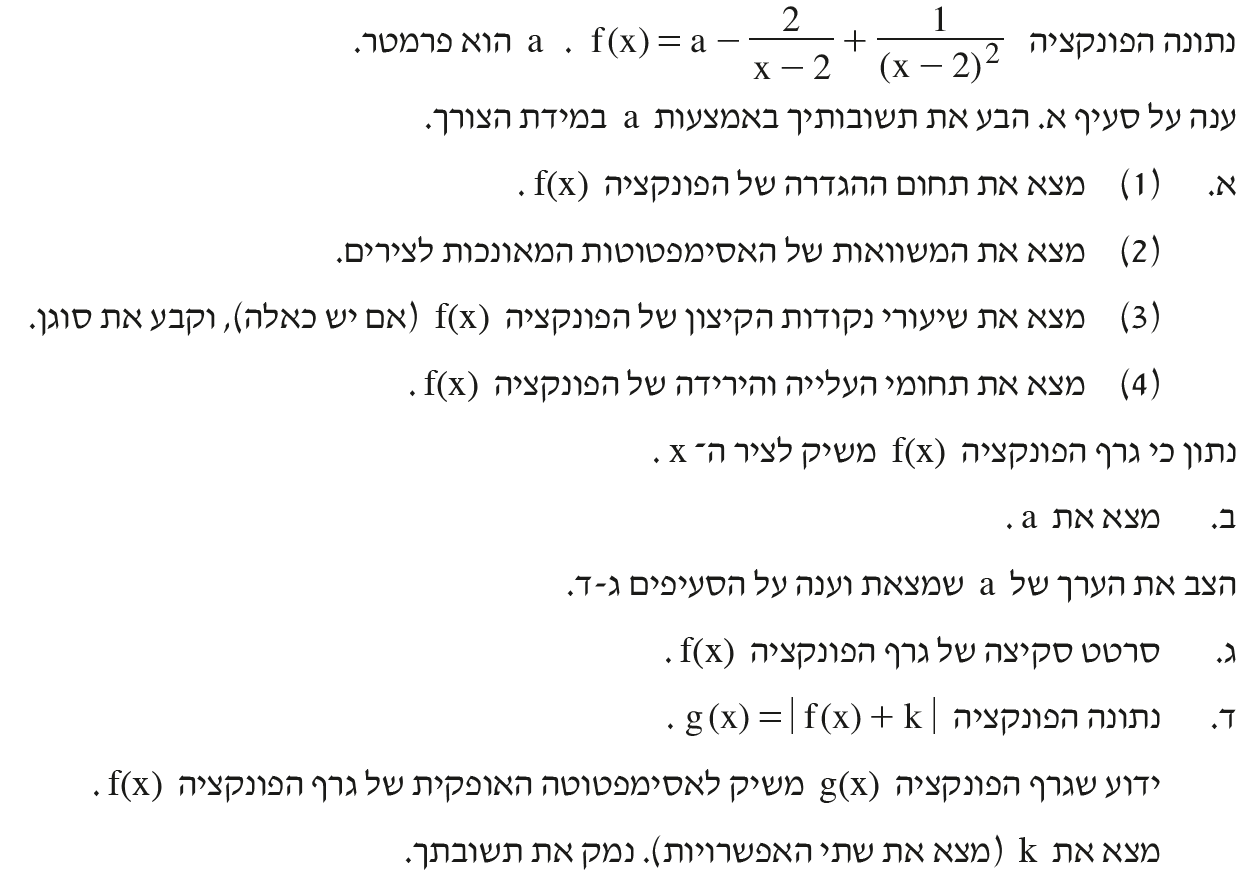
\includegraphics[width=\textwidth]{summer-2017b-6}
\end{center}

\textbf{סעיף א}

$(1)$
תחום ההגדה הוא
$x\neq 2$
כי
$x=2$
מאפס את המכנה של שני גורמים.

$(2)$
כאשר 
$x\rightarrow \pm\infty$
שני גורמים שואפים לאפס, ולכן האסמפטוטה האופקית היא
$y=a$.

כאשר 
$x\rightarrow \pm 2$
שני גורמים שואפים לאינסוף, ולכן האסמפטוטה האנכית היא
$x=2$.

בעתיד בוודאי נצטרך לקבוע את סימן הפונקציה השואפת לאינסוף, אז נחשב בותו כאן. כאשר
$x\rightarrow 2$,
$\disfrac{1}{(x-2)^2}\gg\disfrac{2}{x-2}$
כך ש-%
$y\rightarrow+\infty$
גם מימין וגם משמאל.

$(3)$
\[
f'(x) = -\frac{2\cdot -1}{(x-2)^2} + \frac{-2}{(x-2)^3}=0\,.
\]
הפוקציה לא מוגדרת ב-% 
$x=2$,
כך שאפשר להכפיל את המשוואה ב-%
$(x-2)^3$.
נקבל
$2(x-2)=2$
ו-%
$x=3$.
נקודת הקיצון היא
$(3,a-1)$.

על ידי הכפלות, הנגזרת הראשונה היא:
\[
f'(x) = \frac{2(x-2)^2-2(x-2)}{(x-2)^4}=\frac{2x^2-10x+12)}{(x-2)^4}\,.
\]
המכנה חיובי לכן הסימן של הנגזרת השנייה הוא הסימן נגזרת המונה
$4x-10$.
ב-%
$x=3$,
הסימן חיובי והנקודה היא מינימום.

דרך אחרת לבדוק אם מדובר במינימום או מקסימום היא באמצעות טבלת עליות וירידות:
\[
\begin{array}{c|c|c|c|c|c}
x & 0 & 2 & 2.5 & 3 & 4\\\hline
f'(x) & 0.75 & \times & -0.5& 0 & 0.25\\\hline
f(x) & \nearrow & \times & \searrow & a-1 & \nearrow
\end{array}
\]
הנקודה
$(3,a-1)$
היא מינימום.

$(4)$
ראו בסעיף הקודם.

\textbf{סעיף ב}

ערך ה-%
$y$
בנקודת המינימום הוא אפס.
$f(3)=a-1=0$
ו-%
$a=1$.

\textbf{סעיף ג}

\begin{center}
\selectlanguage{english}
\begin{tikzpicture}[scale=1]
\begin{axis}[
    xlabel = $x$,
    ylabel = {$f(x)$},
    axis lines=center,
    xtick={-2,...,7},
    ytick={-1,...,5},
    xmin = -2,
    xmax = 7,
    ymin = -1,
    ymax = 5,
    xticklabel style={
    anchor=north east,
    },
    yticklabel style={
    anchor=south east,
    },
    every axis y label/.style={at={(ticklabel cs:0.7)},rotate=90,anchor=west,},
    every axis x label/.style={at={(ticklabel cs:0.7)},anchor=north,},
]
\addplot [
    domain=-2:1.3, 
    samples=40, 
]
{1-(2/(x-2))+(1/(x-2)^2)};
\addplot [
    domain=2.3:7, 
    samples=40, 
]
{1-(2/(x-2))+(1/(x-2)^2)};
\draw[dashed,thick] ({axis cs:2,0}|-{rel axis cs:0,0}) -- ({axis cs:2,0}|-{rel axis cs:0,1});
\draw[dashed,thick] ({axis cs:-2,1}-|{rel axis cs:0,0}) -- ({axis cs:-2,1}-|{rel axis cs:7,0});
\fill (axis cs:3,0) circle(1.5pt);
\end{axis}
\end{tikzpicture}
\end{center}


\textbf{סעיף ד}
האסמטוטה האופקית היא
$y=a=1$
ונקודת המינימום של
$f(x)$
היא
$(3,a-1)=(3,0)$:
\begin{eqnarray*}
g(3)&=&|f(3)+k|=a=1\\
|0+k|&=&1\\
k&=&\pm 1\,.
\end{eqnarray*}

\np

\section{המלצות}


\selectlanguage{english}

